\subsection{Почти равномерная сходиость}
\begin{note}
    Зафиксируем некоторое пространство с полной мерой, т.е. тройку $(X, \MM, \mu)$ такую, что $X$~---~абстрактное множество, $\MM$~---~сигма-алгебра его подмножеств, а $\mu$~---~полная счётно-аддитивная мера на $\MM$.
\end{note}

\begin{reminder} (Из 2 семестра)
    Будем говорить, что последовательность  $\{f_n\}_{n = 1}^\infty$ равномерно сходится к $f : X \rightarrow \R,$ если
    $$\forall \epsilon > 0 \ \exists N \in \N: \ \forall n \geq N, \ \forall x \in X: \ |f_n(x) - f(x)| < \epsilon$$
\end{reminder}
\begin{definition} (Почти равномерная сходимость)
    Будем говорить что последовательность $\{f_n\} \subset \LL_0(X, \MM)$ сходится почти равномерно к $f \in \LL_0(X, \MM)$, если $\forall \varepsilon > 0 \  \exists E_\epsilon \in \MM$ такое, что $\mu(E_\epsilon) < \epsilon$ и $f_n \underset{X \setminus E_\epsilon}{\rr} f$ и обозначать это как $f_n \overset{\text{п.р.}}{\underset{X}{\rr}}f, n \ra \infty.$
\end{definition}

\begin{lemma}[Бореля-Кантелли]
    Пусть $\{E_n\} \subset \MM$: $\sum\limits_{n = 1}^\infty \mu(E_n) < +\infty$. Тогда $$\mu\left(\overline{\lim\limits_{n\to \infty}} E_n\right) = \mu\left( \bigcap\limits_{n = 1}^\infty \bigcup\limits_{k \geq n}^\infty E_k\right) = 0.$$
\end{lemma}
\begin{proof}
    Идея в том, что если ряд сошелся, то <<размеры>> множеств стремятся к нулю.\\
    Распишем это формально:
    Если $\sum\limits_{n = N}^\infty \mu(E_n) \rightarrow 0, N \rightarrow \infty$, то: \[ 0 \leq \mu \Bigg(\bigcap\limits_{i = 1}^\infty \bigcup\limits_{k \geq i}^\infty E_k \Bigg) \leq \mu \Bigg(\bigcap\limits_{i = 1}^N \bigcup\limits_{k \geq i}^\infty E_k \Bigg) \leq \mu \Bigg(\bigcup\limits_{k = N}^\infty E_k \Bigg) \leq \sum\limits_{k = N}^\infty \mu(E_k) \rightarrow 0, N \rightarrow \infty\]
    Первое неравенство верно, так как мера не отрицательна.\\
    Второе~---~так как <<если из пересечения что-то выкинуть не станет больше>>.\\
    Третье получается, если взять $i = n$ и $i = n+1$, легко заметить, что их пересечение равносильно тому, чтобы выкинуть $E_n$.\\
    Четвертое~---~в силу счетной полуаддитивности.\\ Далее из теоремы о двух милиционерах получаем искомое.
    Значит $\mu(\overline{\lim\limits_{n \to \infty}} E_n) = 0$.
\end{proof}

\begin{corollary}[Признак сходимости почти всюду и почти равномерно]
    Пусть $\{g_n\} \subset \LL_0(X, \mu)$ такая, что $\forall n \in \N \hookrightarrow \ g_n \geq 0$. И дана бесконечно малая положительная числовая последовательность $\{\epsilon_n\}$. Определим $X_n = X(g_n > \varepsilon_n)$.\\
    Если $\sum\limits_{n = 1}^\infty \mu(X_n) < +\infty$, то выполнено:\\
    1. $g_n \xrightarrow[X]{\text{п.в.}} 0,\  n\rightarrow +\infty$;\\
    2. Более того, $g_n \overset{\text{п.р.}}{\underset{X}{\rr}} 0,\  n \rightarrow +\infty$.\\
\end{corollary}
%%%ВОТ ТУТ
\begin{note}
    Идея в том, что если положительная числовая последовательность $\{\epsilon_n\}$ бесконечно мала, то, чтобы ряд из множеств, где значения $g_n(x) > \varepsilon_n$, стремился к нулю, нужно, чтобы $n$-ый остаток ряда стремился к нулю.
\end{note}
\begin{proof}
    Фиксируем $\epsilon > 0$. Пусть $E_n(\epsilon) = X(g_n > \epsilon)$. Так как $\{\epsilon_n\}$~---~стремится к нулю, то $\exists N_0$: $\varepsilon_{N_0} <  \varepsilon$, и тогда начиная с него $E_n (\epsilon) \subset X_n$. Тогда первые $N_0$ не влияют на сходимость. А из сходимости ряда  $\sum\limits_{n = N_0}^\infty \mu(X_n) < +\infty$ и из монотонности меры следует $\sum\limits_{n = N_0}^\infty \mu(E_n) < +\infty$. \\

    Пусть $x \notin \overline{\lim\limits_{n\to \infty}} E_n$. Тогда $\exists N \in \N$: $x \notin E_n \forall n \geq N$. Но это значит, что $0 \leq g_n(x) \leq \epsilon \  \forall n \geq N$. Тогда, если мы возьмём $\epsilon_k = 1/k$, то так как в силу леммы Бореля-Кантелли $\mu(\overline{\lim\limits_{n\to \infty}} E_n(\epsilon_k)) = 0$, то для $F = \bigcup\limits_{k = 1}^\infty \overline{\lim\limits_{n\to \infty}} E_n(\epsilon_k)$ верно следующее: $x \notin F \Rightarrow g_n(x) \rightarrow 0, n \rightarrow +\infty$. Значит, поскольку $F$~---~множество меры нуль, то $g_n \xrightarrow[X]{\text{п.в.}} 0,\  n\rightarrow +\infty$. \\
    Теперь покажем п.р. сходимость $\{ g_n\}$. Если мы зафиксируем $\epsilon > 0$, то $\exists N(\epsilon) \in \N$: $\sum\limits_{n = N(\epsilon)}^\infty \mu(X_n) < \epsilon$.\\
    Тогда возьмём в качестве $E_\epsilon = \bigcup\limits_{k = N(\epsilon)}^\infty X_k$. Если $x \notin E_\epsilon$, то $\forall n \geq N\ \forall x\in X \hookrightarrow g_n(x) < \epsilon_n$. Тогда поскольку $\epsilon_n$~---~бесконечно малая, то $\sup\limits_{X} g_n (x) \rightarrow 0,  n\rightarrow +\infty$, а значит $g_n$ равномерно сходится на $X \setminus E_\epsilon$. Значит есть п.р. сходимость на $X$.
\end{proof}
\subsection{Теоремы Рисса и Егорова}
\begin{theorem}[Рисс]
    Пусть дана последовательность $\{f_n\} \subset \LL_0(X, \mu)$, сходящаяся по мере к некоторой $f \in \LL_0(X, \mu)$. Тогда у неё существует подпоследовательность $f_{n_k} \xrightarrow[X]{\text{п.в.}} f, k \rightarrow +\infty$
\end{theorem}
\begin{proof}
    Так как $f_n$ сходится к $f$ по мере, то $\forall \epsilon > 0 \hookrightarrow \mu(\{x \in X \mid |f_n(x) - f(x)| \geq \epsilon\}) \rightarrow 0, n \rightarrow +\infty$. Тогда $\forall k \in \N \  \exists n_k$: \[\mu\left(\{x \in X \mid |f_{n_k}(x) - f(x)| \geq \frac{1}{k}\}\right) \leq \frac{1}{2^k}\]
    Тогда $\sum\limits_{k = 1}^\infty \mu(\{x \mid |f_{n_k}(x) - f(x)| \geq \frac{1}{k}\}) < +\infty$, а значит применяя следствие из леммы Бореля-Кантелли, мы получаем, что $\{ f_{n_k} \}_{k = 1}^{\infty}$  п.в. сходится к $f$; более того, $\{ f_{n_k} \}_{k = 1}^{\infty}$ п.р. сходится к $f$.
\end{proof}

\begin{theorem}[Егоров]
    Пусть даны $E \in \MM$: $\mu(E) < +\infty$ и последовательность $\{f_n\} \subset \LL_0(E, \mu)$. Тогда если последовательность сходится п.в. к $f \in \LL_0(E, \mu)$, то она сходится п.р.
\end{theorem}
\begin{proof}
    Пусть $g_n  = \sup\limits_{k \geq n} |f_k - f|$. По условию, $g_n \xrightarrow[E]{\text{п.в.}} 0, n \rightarrow +\infty$. Поскольку мера пространства конечна, то из сходимости п.в. следует сходимость по мере (согласно теореме Лебега). Тогда по теореме Рисса существует подпоследовательность $g_{n_k}$, сходящаяся п.р к $0, k \rightarrow +\infty$. Покажем, что из этого следует, что и вся $g_n$ сходится п.р. \[\forall \epsilon > 0 \exists E_\epsilon: \mu(E_\epsilon) < \epsilon \hookrightarrow g_{n_k} \underset{E \setminus E_\epsilon}{\rr} 0\]
    Что означает сходимость равномерно на $E_\epsilon?$ То, что $\sup\limits_{x\in E \setminus E_\epsilon} |g_{n_k} (x)| \rightarrow 0, k \rightarrow +\infty$. Но последовательность $g_n$~---~монотонна. А значит $\sup\limits_{x\in E \setminus E_\epsilon} |g_{n_k} (x)| \rightarrow 0, n \rightarrow +\infty$, то есть $g_n \underset{E \setminus E_\epsilon}{\rr} 0$. Но тогда поскольку $|f_n - f| \leq g_n$, то $f_n \underset{E \setminus E_\epsilon}{\rr} f$, $n\to \infty$, то есть мы получаем п.р. сходимость к $f$.
\end{proof}

\begin{lemma}
    Пусть $X$~---~пространство с $\sigma$-конечной мерой $\mu$. Тогда существует конечная мера $\nu$, уважающая множества меры нуль, т.е. $\mu(E) = 0 \Longleftrightarrow \nu(E) = 0$
\end{lemma}
\begin{proof}
    Поскольку $X$~---~пространство с $\sigma$-конечной мерой, то $X = \bigsqcup\limits_{k = 1}^\infty X_k$, где мера каждого из $X_k$~---~конечна. Тогда определим $\nu$ как \[\nu(E) = \sum\limits_{k = 1}^\infty \frac{1}{2^k} \frac{\mu(E \cap X_k)}{\mu(X_k)}\]
    Очевидно, что $\nu$ удовлетворяет требованиям.
\end{proof}

\begin{theorem}[о диагональной последовательности]
    Пусть $X$~---~пространство с $\sigma$-конечной мерой. Тогда если есть $\{g_n\} \subset \LL_0(X, \mu)$, сходящаяся п.в. к $h \in \LL_0(X, \mu)$ и $\forall n \in \N$ есть $\{f_{n,k}\} \subset \LL_0(X, \mu)$ сходящаяся п.в. к $g_n$, то $\forall n \in \N \ \exists k(n) \in \N$ такая, что $f_{n, k(n)} \xrightarrow[X]{\text{п.в.}} h, n \rightarrow +\infty$.
\end{theorem}
\begin{proof}
    Предположим, что $\mu(X) < +\infty$. Тогда по теореме Лебега из сходимости п.в. следует сходимость по мере, то есть $\forall n \in \N \hookrightarrow f_{n, k} \xrightarrow{\mu} g_n, k \rightarrow +\infty$. То есть $$\forall n \in \N \ \exists E_n = \left\{x \mid |f_{n, k(n)} - g_n| > \frac{1}{n}\right\}: \text{ } \mu(E_n) < \frac{1}{2^n}.$$ Тогда заметим, что $\sum\limits_{n = 1}^\infty \mu(E_n) < +\infty$, а значит, применяя следствие из леммы Бореля-Кантелли, мы получаем, что $\psi_n = f_{n, k(n)} - g_n$ сходится к нулю п.в. Тогда $h - f_{n, k(n)} = h - g_n - \psi_n$. Поскольку $h - g_n$  п.в. сходится к нулю, и $\psi_n$ п.в. сходится к нулю, то и $h - f_{n, k(n)}$ п.в. сходится к нулю, то есть $f_{n, k(n)} \xrightarrow{\text{п.в.}} h, n \rightarrow +\infty$.
    Пусть теперь $X$~---~пространство с $\sigma$-конечной мерой. Тогда мы применяем ранее доказанное к $(X, \MM, \nu)$, где $\nu$ из леммы $4.2$, и получаем требуемое; а поскольку $\nu$ уважает множества меры нуль, то множество точек отсутствия сходимости сохранит меру нуль.
\end{proof}

\subsection{Теорема Лузина. Аппроксимация измеримых функций непрерывными}
\begin{note}
    Далее работаем в $\R^n$ со стандартной мерой Лебега.
\end{note}

\begin{reminder}
    Расстоянием от точки до множества будем называть число $\rho(x, E) = \inf\limits_{y \in E} \|x - y\|$.
\end{reminder}

\begin{lemma}
    Функция расстояния от точки до множества является $1-$липшицевой.
\end{lemma}
\begin{proof}
    Пусть $x, x' \in \R^n$. Тогда согласно неравенству треугольника, $\|x - y\| \leq \|x - x'\| + \|x' - y\|$.
    Возьмём инфимум по всем $y \in E:$ \[\rho(x, E) \leq \|x - x'\| + \rho(x', E).\]
    Поскольку это верно для произвольных $x, x'$, то справедливо следующее: \[|\rho(x, E) - \rho(x', E)| \leq \|x - x'\|.\]
    То есть $\rho$~---~1-липшицева.
\end{proof}

\begin{lemma}
    Пусть $K_0, K_1$~---~непересекающиеся компакты в $\R^n$. Тогда существует непрерывная функция $h_{K_0, K_1}$, разделяющая $K_0$ и $K_1$, то есть $\forall x \in K_0 \hookrightarrow h(x) = 0, \forall x \in K_1 \hookrightarrow h(x) = 1$.
\end{lemma}
\begin{proof}
    Положим \[h_{K_0, K_1}(x) = \dfrac{\rho(x, K_0)}{\rho(x, K_0) + \rho(x, K_1)} > 0.\]
    Очевидно, что эта функция удовлетворяет всем условиям леммы.
\end{proof}

\begin{theorem}
    Пусть $K \subset \R^n$~---~компакт. Тогда существует $\{f_n\}$~---~последовательность непрерывных функций, сходящаяся к $\chi_K$.
\end{theorem}
\begin{proof}
    Заметим, что $G = \R^n \setminus K$~---~открытое, а значит измеримое. Тогда из регулярности меры Лебега следует возможность исчерпать $G$ компактами: $G = \bigcup\limits_{n \in \N} K_n$, причём $\forall n \in \N \hookrightarrow K_n \subset K_{n + 1}$. Таким образом, взяв $f_n = h_{K_n, K}$ мы получаем искомую последовательность непрерывных функций: очевидно, что любая точка вне $K$ начиная с некоторого $N$ окажется в $K_N$ и после этого $f_n(x)$ будет равен 0; для любой точки компакта значение функции всегда равно 1.
\end{proof}



\begin{theorem}[Теорема Фреше/2 теорема Рисса]
    Пусть $h$~---~произвольная измеримая функция на $X$. Тогда существует последовательность $\{f_n\} \subset C(\R^n)$: $f_n \xrightarrow[\R^n]{\text{п.в.}} h, n \rightarrow +\infty$
\end{theorem}
\begin{proof}
    Докажем теорему в несколько шагов. \\
    Пусть $\phi$~---~харфункция некоторого измеримого множества $E$. Согласно внутренней регулярности меры Лебега, его можно исчерпать компактами: $E = \bigcup\limits_{n \in \N} K_n$, т.ч. $K_n \subset K_{n + 1}$. Тогда поскольку $\forall n \in \N$ мы можем аппроксимировать харфункцию компакта непрерывными, и харфункции компактов сходятся к харфункции $E$, то в силу $\sigma$-конечности $\R^n$ по теореме о диагональной последовательности $\exists \{g_{n, k(n)}\}_{n = 1}^{\infty}$: $g_{n, k(n)} \xrightarrow{\text{п.в.}} \chi_E, n \rightarrow +\infty$, и все $g_{n, k(n)}$~---~непрерывные на $\R^n$.\\
    Пусть теперь $\psi$~---~некоторая простая функция; Очевидно, что она также аппроксимируется непрерывными функциями, поскольку является суммой харфункций некоторых дизъюнктных измеримых множеств. \\
    Пусть теперь $h$~---~произвольная измеримая функция. Тогда существует последовательность простых функций $\{g_n\}$ т.ч. $g_n \rightarrow h, n \rightarrow +\infty$. В тоже время, $\forall n\ \in \N$ существует $f_{n, k} \xrightarrow{\text{п.в.}} g_n, k \rightarrow +\infty$~---~последовательность непрерывных функций. В силу сигма-конечности $\LL^n$ мы можем применить теорему о диагональной последовательности и получить $f_{n, k(n)} \xrightarrow[\R^n]{\text{п.в.}} h, n \rightarrow +\infty$. 
\end{proof}

\begin{definition}
    \textit{$C$-свойством Лузина} будем называть следующее условие на функцию: \[\forall \epsilon > 0 \ \exists E_\epsilon: \LL^n(E_\epsilon) < \epsilon \wedge \exists f_\epsilon \in C(\R^n \setminus E_{\epsilon}) \  \forall x \in \R^n \setminus E_\epsilon \hookrightarrow f(x) = f_\epsilon(x).\]
\end{definition}

\begin{theorem}[Лузина]
    Произвольная измеримая п.в. конечная функция $f$ в $\R^n$ удовлетворяет $C$-свойству Лузина.
\end{theorem}
\begin{proof}
    Заметим, что \[\R^n = \bigcup\limits_{m = 1}^\infty B_m(0) \setminus \overline{B_{m - 1}(0)} \cup \bigcup\limits_{i = 1}^\infty S_i(0) \cup \{ 0\}.\]
    По теореме Фреше существует последовательность $\{f_l\} \subset C(\R^n)$: $f_l \xrightarrow[\R^n]{\text{п.в.}} f, l \rightarrow +\infty$. В тоже время, поскольку мера каждого шарового слоя -- конечна, то мы можем применить теорему Егорова на каждом из них, и получить п.р. сходимость на каждом из них, то есть \[\forall m \in \N \exists e_m \subset E_m \hookrightarrow f_l \underset{E_m \setminus e_m}{\rr} f, l \rightarrow +\infty,\]
    причём $\mu(e_m) \leq \frac{\epsilon}{2^m}$.
    Но тогда $\LL^n(\bigcup\limits_{i = 1}^\infty e_i) \leq \epsilon$. Тогда мы можем взять $E_\epsilon = \bigcup\limits_{m = 1}^\infty e_m \cup \bigcup\limits_{i = 1}^\infty S_i$. Очевидно, что на всё остальном пространстве $f_l$ сходится к $f$ равномерно, а следовательно $f$ непрерывно на нём, таким образом мы получаем утверждение задачи.
\end{proof}

\section{Интеграл Лебега}
\subsection{Определение интеграла Лебега и его корректность}
\begin{reminder}
    Простая функция~---~функция с конечным числом значений.
\end{reminder}
\begin{definition}[Интеграл Лебега Toy version 1]
    Пусть $f$~---~простая неотрицательная функция. Тогда интегралом Лебега на множестве $E$ от неё будем называть \[\int\limits_E fd\mu = \sum\limits_{k = 1}^N a_k\mu(E_k \cap E) \in [0, +\infty]\]
\end{definition}
\begin{definition}
    Простую неотрицательную функцию $f$ будем называть \textit{интегрируемой по Лебегу}, если интеграл от неё конечен.
\end{definition}
\begin{lemma}
    Определение интеграла Лебега для простой функции корректно, то есть интеграл Лебега не зависит от разбиения.
\end{lemma}
\begin{proof}
    Пусть $X = \bigsqcup\limits_{i = 1}^N E_i = \bigsqcup\limits_{j = 1}^M F_j$ и простая неотрицательная функция $f = \sum\limits_{i = 1}^N a_i\chi_{E_i} = \sum\limits_{j = 1}^M b_j\chi_{F_j}$. Заметим, что $\{E_i \cap F_j\}_{i, j}$~---~допустимое разбиение для $f$, $E_i \cap E = \bigsqcup\limits_{j = 1}^M E_i \cap F_j \cap E$. Тогда \[\sum\limits_{i = 1}^N a_i\mu(E \cap E_i) = \sum\limits_{i = 1}^N\sum\limits_{j = 1}^M a_i\mu(E \cap E_i \cap F_j) = \]\[=  \sum\limits_{i = 1}^N\sum\limits_{j = 1}^M b_j\mu(E \cap E_i \cap F_j) = \sum\limits_{j = 1}^M\sum\limits_{i = 1}^N b_j\mu(E \cap E_i \cap F_j) = \sum\limits_{j = 1}^M b_j\mu(E \cap F_j)\]
\end{proof}


\begin{definition}[Интеграл Лебега Toy version 2]
    Пусть $f$~---~неотрицательная измеримая функция. Тогда \[\int\limits_E fd\mu = \sup\limits_{0 \leq \psi \leq f} \int\limits_E \psi d\mu,\]
    где супремум берётся по всем таким простым функциям $\psi$.
\end{definition}

\begin{minipage}{0.5\textwidth}% adapt widths of minipages to your needs
    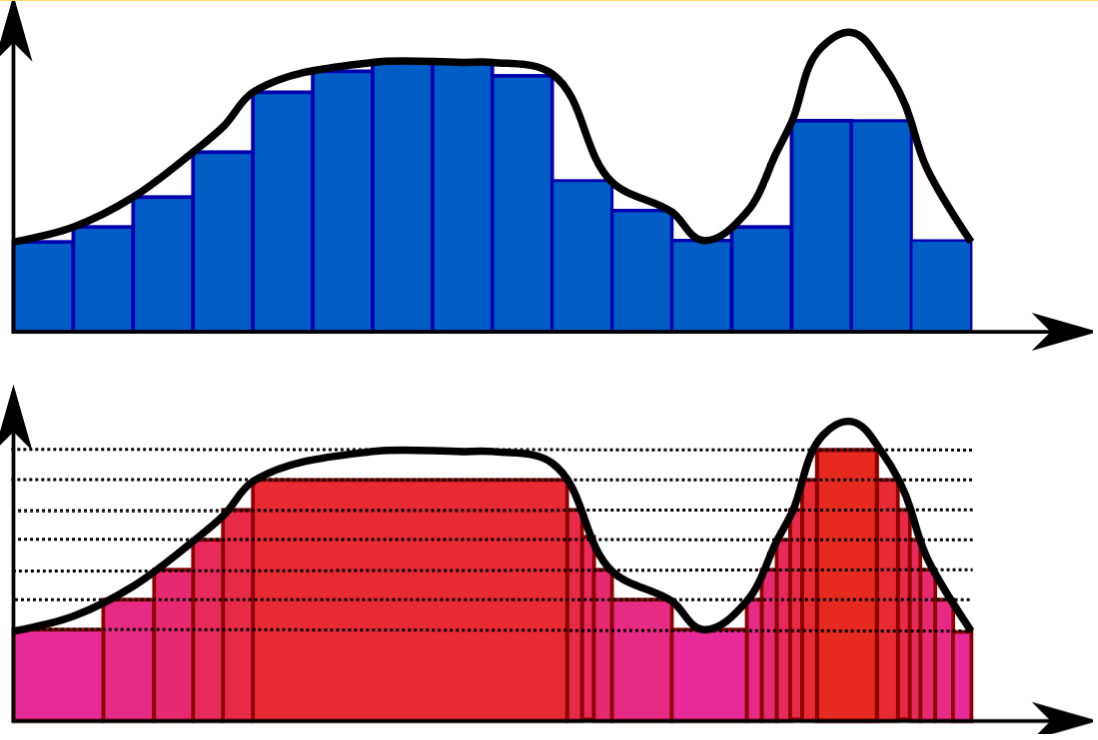
\includegraphics[width=0.9\textwidth]{images/Screenshot_7.png} 
\end{minipage}%
 \hfill%
 \begin{minipage}{0.5\textwidth}\raggedright
Пояснение к картинке. Синий цвет~---~это сумма Дарбу, разбиение по области определения.\\ А красный~---~это сумма Лебега. Мы приближаем нашу функцию простыми, разбиение по оси значений функции.
 \end{minipage}


\begin{definition}[Интеграл Лебега]
    Пусть $f$~---~произвольная измеримая на $E$ функция. Тогда $f = f_+ - f_-$, где $f_+ = \max(f, 0), f_- = \max(-f, 0)$. Определим \textit{интеграл Лебега} от неё как \[\int\limits_E fd\mu = \int\limits_E f_+d\mu - \int\limits_E f_-d\mu,\] в случае конечности интегралов от неотрицательных частей. Иначе будем говорить что функция $f$ \underline{не интегрируема} по Лебегу.
\end{definition}
\begin{definition}
    Произвольную измеримую функцию $f$ будем называть \textit{интегрируемой по Лебегу}, если $\int\limits_E f_+d\mu < +\infty$ и $\int\limits_E f_-d\mu < +\infty$.
\end{definition}

\subsection{Неравенства Гёльдера, Минковского и Чебышёва. Пространства $L_p$}
Пусть $X = (X, \MM, \mu)$~---~пространство с мерой.
\begin{definition}
    Пусть $p \in [1, +\infty), E \in \MM$. Тогда положим:\[\widetilde{L_p}(E, \mu) = \{f \in \LL_0(E, \mu) \Big | \ \int\limits_E |f|^pd\mu < +\infty\}\]
\end{definition}
\begin{lemma}[Неравенство Юнга]
    $\forall a, b \geq 0 \hookrightarrow $
    \[ab \leq a^p/p + b^{p'}/p',\text{ где }1/p + 1/p' = 1.\]
\end{lemma}
\begin{proof}
    Из выпуклости логарифма вверх  мы можем оценить
    $$\ln(a^p/p + b^{p'}/p') \geq \ln(a^p)/p + \ln(b^{p'})/p' = \ln a + \ln b = \ln ab$$ Потенцируем и получим исходное неравенство:
    \[ab \leq \dfrac{a^p}{p} + \dfrac{b^{p'}}{p'}\]
\end{proof}

\hypertarget{gyolder}{}
\begin{theorem}[Неравенство Гёльдера]
    Пусть $f \in \widetilde{L_p}(E, \mu), g \in \widetilde{L_{p'}}(E, \mu)$, где $p, p' \in (1, +\infty)$: $\frac{1}{p} + \frac{1}{p'} = 1$. Тогда $(f\cdot g) \in \widetilde{L_1}$ и \[\int\limits_E |fg|d\mu \leq \Bigg(\int\limits_E |f|^p d\mu\Bigg)^{1/p}\Bigg(\int\limits_E |g|^{p'}d\mu \Bigg)^{1/{p'}}\]
\end{theorem}

\begin{proof}
        Пусть $A = (\int\limits_E |f|^pd\mu)^{1/p}, B = (\int\limits_E |g|^{p'}d\mu)^{1/p'}$. Предположим, что $A > 0$ и $B > 0$ (случаи, когда $A = 0$ или $B = 0$ тривиальны). Нормируем $\widetilde{f} = f/A, \widetilde{g} = g/B$. Тогда \[\Bigg(\int\limits_E |\widetilde{f}|^p d\mu \Bigg)^{1/p} = \Bigg(\int\limits_E |\widetilde{g}|^{p'} d\mu\Bigg)^{1/p'} = 1\]
    Используя неравенство Юнга \[\int\limits_E |\widetilde{f}\widetilde{g}|d\mu \leq \int\limits_E {\Bigg(\dfrac{|\widetilde{f}|^p}{p} + \dfrac{|\widetilde{g}|^{p'}}{p'}\Bigg)}d\mu = \dfrac{1}{p}\int\limits_E |\widetilde{f}|^pd\mu + \frac{1}{p'}\int\limits_E |\widetilde{g}|^{p'}d\mu = 1.\]
    Теперь, домножив на $A$ и $B$, мы получаем искомое.
\end{proof}



\begin{note}
    В доказательстве неравенства Гёльдера используются свойства интеграла Лебега, показанные далее в п. $5.3$.
\end{note}

\begin{reminder}
    Если $p \in [1, +\infty)$, то обозначим
    \[\widetilde{L_p}(E, \mu) = \{f: E \rightarrow \overline{\R} \Big | f\text{~---~измерима в широком смысле на}\ E, \int\limits_{E} |f|^pd\mu < +\infty\}\]
\end{reminder}

\begin{note}
    Обозначим за $\mathcal{N}(E)$~---~линейное пространство всех измеримых в широком смысле функций на $E$, т.ч. они равны 0 п.в. и <<выкинем>> их. Это сделано, чтобы у нас не страдала аксиома нормы связанная с нулем(Мы поменяли функцию на множестве меры нуль, и получили нулевой интеграл)
    Тогда:\\ \[L_p(E, \mu) = \widetilde{L_p}(E, \mu)/\mathcal{N}(E)\]
    Является ЛНП с нормой \[ \|f\|_p = \Bigg(\int\limits_{E} |f|^p d\mu\Bigg)^{1/p}\]
    \begin{note}
        $L_p$ - это фактор пространство, те его элемент 
    то класс эквивалентности $[f] = f + \mathcal{N}(E)$
    \end{note} 

    
    Проверим выполнение аксиом нормы: 
    \begin{itemize}
        \item Не отрицательность очевидна.
        \item $\|f\|_p = 0 \Longleftrightarrow f = 0$~---~в силу факторизации и ранее доказанных свойств.
        \item Неравенством треугольника является неравенство Минковского.
    \end{itemize}
\end{note}

\begin{lemma}[Неравенство Минковского]
    Пусть $f, g \in \widetilde{L_p} (E)$. Тогда $f + g \in \widetilde{L_p} (E)$ и $\|f + g\|_p \leq \|f\|_p + \|g\|_p$.
\end{lemma}
\begin{proof}
    Так как $|f + g|^p \leq (2\max (|f|, |g|))^p \leq 2^p(|f|^p + |g|^p)$, то и $\int\limits_{E} |f + g|^p d\mu < +\infty$, а значит $f + g \in \widetilde{L_p} (E)$. Тогда \[\int\limits_{E} |f + g|^p d\mu = \int\limits_{E} |f + g||f + g|^{p - 1}d\mu \leq \]\[  \leq \int\limits_{E} (|f| + |g|)|f + g|^{p - 1}d\mu = \int\limits_{E} |f||f + g|^{p - 1}d\mu + \int\limits_{E} |g||f + g|^{p - 1}d\mu = \int\limits_{E} |f||f + g|^{p/p'}d\mu + \int\limits_{E} |g||f + g|^{p/p'} d\mu \leq \]  \hyperlink{gyolder}{По неравенству Гёльдера} с показателем $p, p':$ \[
    \leq \left(\int\limits_{E} |f|^pd\mu \right)^{1/p} \left(\int |f + g|^p \right)^{1/p'} + \left(\int\limits_{E} |g|^pd\mu \right)^{1/p} \left(\int\limits_{E} |f + g|^p \right)^{1/p'}.
    \]
    Теперь, поскольку $1/p + 1/p' = 1$, то если мы поделим на $(\int\limits_{E} |f + g|^p)^{1/p'} < +\infty$ обе части, то мы получим необходимое неравенство.
\end{proof}

\begin{definition}
    Будем называть \textit{\underline{существенным супремумом}} для измеримой функции $f$ на пространстве с мерой $(X, \MM, \mu)$ следующее: \[\esssup\limits_{x \in X}|f(x)| = \inf\{L > 0 \mid \mu(|f| > L) = 0\}\]
\end{definition}
\begin{definition}
    Пусть $(X, \MM, \mu)$~---~пространство с мерой. Будем говорить что $f: X \rightarrow \overline{\R}$~---~существенно ограничена, если $\esssup\limits_{x \in X} |f(x)| < +\infty$.
\end{definition}
\begin{definition}
    Определим $L_\infty$ как ЛНП классов эквивалентности существенно ограниченных на $X$ функций с нормой $\esssup$, то есть $\|f\|_\infty = \esssup\limits_X |f|$.
\end{definition}
\begin{note}
    Неравенства Гёльдера и Минковского работают и в этом случае, то есть при $p = 1$/$p = +\infty$.
\end{note}

\begin{theorem}[Неравенство Чебышева]
    Пусть даны положительные $p$ и $t$ и интегрируемая по Лебегу функция $f$. Тогда если $E_t = \{x \in X \mid |f| \geq t\}$, то \[\mu(E_t) \leq \frac{1}{t^p}\int\limits_X |f|^pd\mu\]
\end{theorem}
\begin{proof}
    \[t^p\mu(E_t) = \int\limits_{E_t} t^pd\mu \leq \int\limits_{E_t} |f|^pd\mu \leq \int\limits_{X}|f|^pd\mu\]
\end{proof}